\documentclass[12pt]{report}

%Vous souciez pas de tout les packages, j'ai oublié ce que fait la moitié d'entre eux

\usepackage[utf8]{inputenc}
\usepackage[T1]{fontenc}
\usepackage[francais]{babel}
%\usepackage{layout}
\usepackage[left=3cm,right=3cm,top=3cm,bottom=3cm]{geometry}
%\usepackage{setspace}
\usepackage{soul}
\usepackage[normalem]{ulem}
%\usepackage{eurosym}
%\usepackage{bookman}
%\usepackage{charter}
%\usepackage{newcent}
%\usepackage{lmodern}
%\usepackage{mathpazo}
%\usepackage{mathptmx}
%\usepackage{url}
%\usepackage{verbatim}
%\usepackage{moreverb}
%\usepackage{listings}
%\usepackage{fancyhdr}
%\usepackage{wrapfig}
\usepackage{color}
%\usepackage{colortbl}
\usepackage{amsmath}
\usepackage{amssymb}
\usepackage{mathrsfs}
%\usepackage{asmthm}
%\usepackage{makeidx}
\usepackage{graphicx}
\usepackage{tabularx}
\usepackage{tgtermes}
\usepackage{titlesec}
\usepackage[final]{pdfpages} 
\usepackage{epsfig}
\usepackage{comment}
\usepackage{float}
\usepackage{amsmath}
\renewcommand{\emph}{\textit}
\renewcommand{\thesection}{\arabic{section}}
\renewcommand{\thesubsection}{\arabic{section}.\arabic{subsection}}
\titleformat*{\subsection}{\bfseries}
\parskip=5pt

%Information pour la page de garde

\title{TP1 - Géométrie \'Epipolaire}
\author{Jean-Baptiste \bsc{Morice}, Guillaume \bsc{Versal}}
\date{\today}

\begin{document}

%Commande qui crée la page de garde
\maketitle

\tableofcontents

\newpage
\section*{Introduction}

L'objectif de ce TP est de se familiariser avec les éléments de base de la géométrie épipolaire. On nous fourni dans ce TP deux images représentant la même scène mais avec des points de vu différents. Nous devrons analyser et expliquer les matrices servant à la réalisation de ces images et tracer les différentes droites épipolaires selon des configurations de caméra différente.

\newpage
\section{Notre travail}

\subsection*{Question 1}

Dans le TP, on nous fourni la description de la matrice K. Cette dernière est la matrice de calibration de la caméra et elle se présente comme suit :

\[ K = \begin{pmatrix}
800 & 0 & 200 \\ 
0 & 800 & 150 \\ 
0 & 0 & 1
\end{pmatrix} = 
\begin{pmatrix}
p_x & 0 & u_0 \\ 
0 & p_y & v_0 \\ 
0 & 0 & 1
\end{pmatrix}\]

Les variables $p_x$ et $p_y$ correspondent respectivement à $\frac{f}{l_x}$ et $\frac{f}{l_y}$ avec $f$ étant la distance focale et $l_x$ et $l_y$ la taille du pixel. Les variables $u_0$ et $v_0$, sont quant à elles, la projection orthogonale du centre optique. 

\subsection*{Question 2}

Dans le sujet, on nous fournit la matrice $^{g}\textrm{T}_o$, cette dernière définie la position de la caméra $C_g$. Les matrices définissant la position de la caméra dans l'espace son de la forme :

\[ ^{c}\textrm{T}_w = \begin{pmatrix}
^{c}\textrm{R}_w & ^{c}\textrm{t}_w  \\
 0_{3 \times 1} & 1
\end{pmatrix} \]

En utilisant la matrice $^{g}\textrm{T}_o$ à notre disposition, nous devons définir la matrice $^{d}\textrm{T}_o$ pour positionner la caméra $C_d$ à 10 cm à droite de $C_g$. Cela revient à effectuer une translation de 10 cm sur l'axe $x$. Ainsi, en appliquant cette transformation on obtient :

\[ ^{d}\textrm{T}_o = \begin{pmatrix}
1 & 0 & 0 & 0.1\\ 
0 & 1 & 0 & 0\\ 
0 & 0 & 1 & 2\\
0 & 0 & 0 & 1
\end{pmatrix} \]

\subsection*{Question 3 et 4}

Comme on peut le constater, les matrices $^{d}\textrm{T}_o$ et $^{g}\textrm{T}_o$ sont pratiquement semblable. Leur unique différence est la translation sur l'axe $x$. Ainsi, $C_g$ et $C_d$ sont sur le même plan. Un tel système est un système réctifié. On peut facilement constater cela sur les images $I_g$ et $I_d$ ci-dessous.

\begin{figure}
\begin{center}
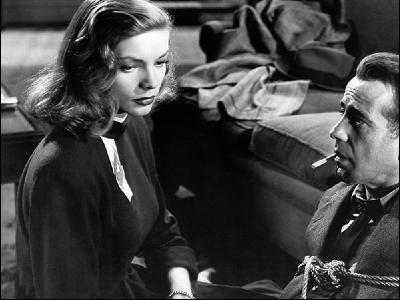
\includegraphics[scale=0.5]{Image/Id.jpg} 
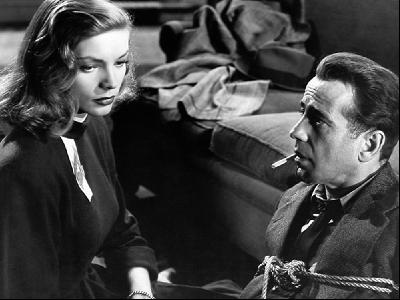
\includegraphics[scale=0.5]{Image/Ig.jpg} 
\caption{Image $I_d$ et $I_g$ réctifiées}
\end{center}
\end{figure}

\subsection*{Question 5 à 8}

On souhaite pouvoir mettre en correspondant un point d'une image dans une autre.Pour trouver les correspondant des points $x_d$ de $I_d$ dans $I_g$, on représente un lieu géométrique qui est une droite d'équation $au_g + bv_g + c = 0$. Pour calculer cette droite on utilise la formule ci-dessous :

\[^{g}\textrm{F}_d \, \bar{x_2} = \, ^{g}\textrm{F}_d \begin{pmatrix}u_d\\ v_d\\ 1\end{pmatrix} = \begin{pmatrix}
a\\ 
b\\ 
c
\end{pmatrix}\] 

Dans le TP, on nous demande de calculer les équations des droites pour les points (100,100) et (50,75), qui correspondent respectivement aux résultats suivant :

\[\begin{matrix}
a = 0,\, b = 0.000125, \,c = -0.0125\\ 
a = 0,\, b = 0.000125,\, c = -0.009375
\end{matrix}\] 

Pour montrer plus clairement ces lieux géométrique sur les images, on les affiches sur l'image $I_g$ et on obtient le résultat ci-dessous.

Comme on peut l'observer sur les images, les droites épipolaires sont parallèles entre elles et par rapport à l'axe $x$. De plus, les points mis en correspondance avec une droite sont au même niveau que celle-ci. 

\begin{figure}[H]
\begin{center}
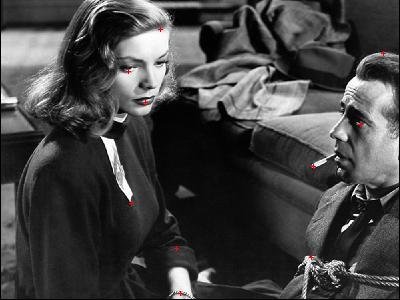
\includegraphics[scale=0.5]{Image/I1d.jpg} 
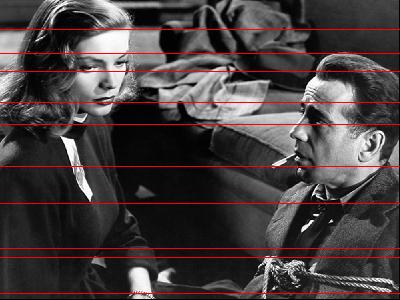
\includegraphics[scale=0.5]{Image/I1g.jpg} 
\caption{Image $I_d$ et $I_g$ avec lieu géométrique}
\end{center}
\end{figure}

Lorsque l'on fait le processus dans le sens inverse, on obtient le même résultat dans l'image $I_d$ que ce que l'on pouvait observer sur l'image $I_g$

\begin{figure}[H]
\begin{center}
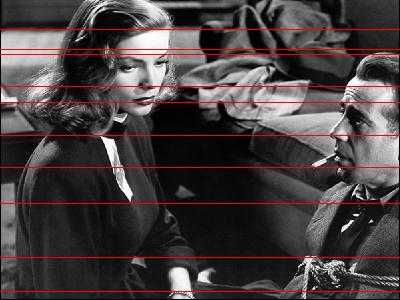
\includegraphics[scale=0.5]{Image/I2d.jpg} 
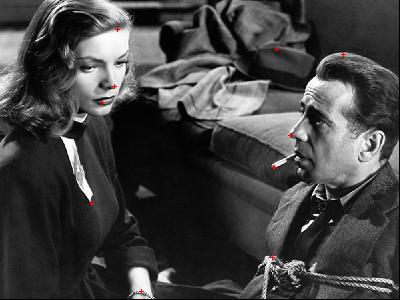
\includegraphics[scale=0.5]{Image/I2g.jpg} 
\caption{Image $I_d$ et $I_g$ avec lieu géométrique (inversion processus)}
\end{center}
\end{figure}

Comme les faisceaux d'épipolaires sont parallèles dans les deux images, ont peu en tirer la conclusion que les deux épipoles sont à l'infini.

\subsection*{Question 9 à 11}

Pour cette partie du TP, on nous demande de mettre la caméra $C_g$ 20 cm devant la caméra $C_d$. Cela revient à reprendre la matrice $^{d}\textrm{T}_o$ et à modifier seulement la translation en $z$. Nous obtenons le résultat ci-dessous :

\[ ^{g}\textrm{T}_o = \begin{pmatrix}
1 & 0 & 0 & 0\\ 
0 & 1 & 0 & 0\\ 
0 & 0 & 1 & 1.8\\
0 & 0 & 0 & 1
\end{pmatrix} \]

Comme il n'y a pas de de translation en $x$ ou en $y$, les épipoles sont confondus sur l'axe $z$

Dans le TP, on nous demande de calculer les équations des droites pour les points (100,100) et (50,75), qui correspondent respectivement aux résultats suivant :

\[\begin{matrix}
a = -1.5625e-05,\, b = 3.125e-05, \, c = -0.0015625\\ 
a = -2.34375e-05,\, b = 4.6875e-05,\, c = -0.00234375
\end{matrix}\] 

On peut observer sur les images que les droites se croisent en un point unique. 


\begin{figure}[H]
\begin{center}
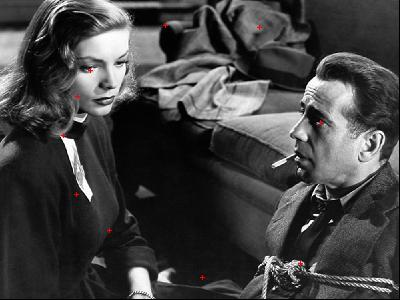
\includegraphics[scale=0.5]{Image/I3d.jpg} 
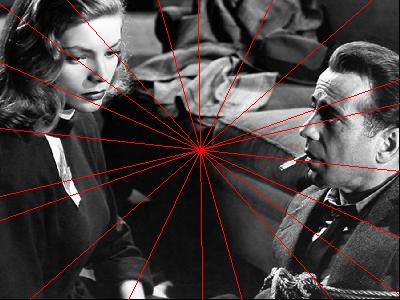
\includegraphics[scale=0.5]{Image/I3g.jpg} 
\caption{Image $I_d$ et $I_g$ avec lieu géométrique ($C_g$ devant $C_d$)}
\end{center}
\end{figure}

\subsection*{Question 12 à 14}

Pour cette partie du TP, on nous demande de mettre la caméra $C_d$ 20 cm dans une certaine configuration. C'est pour cette raison que 

Dans le TP, on nous demande de calculer les équations des droites pour les points (100,100) et (50,75), qui correspondent respectivement aux résultats suivant :

\[\begin{matrix}
aa = -0.0002074345019, \,b = -0.0001004198244,\, c = 0.02391983064\\ 
a = -0.0002034039049, \,b = -0.0001087370748, \,c = 0.01220298122
\end{matrix}\] 

Dans le cas présent, on retrouver une configuration générale pour les épipoles. Les lignes sur l'image paraisse parallèles mais elles ne le sont pas et on peut observer qu'elles s'éloignent petit à petit les unes des autres.

\begin{figure}[H]
\begin{center}
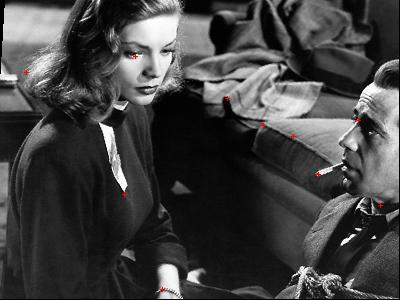
\includegraphics[scale=0.5]{Image/I4d.jpg} 
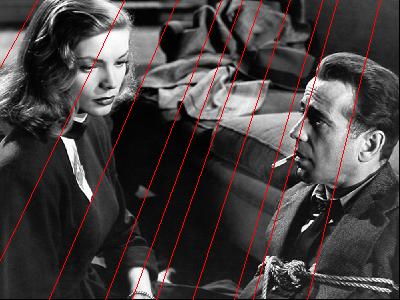
\includegraphics[scale=0.5]{Image/I4g.jpg} 
\caption{Image $I_d$ et $I_g$ avec lieu géométrique (avec rotation et translation)}
\end{center}
\end{figure}

\section{Conclusion}

Ce TP nous a permis de nous familiariser avec les éléments de base de la géométrie épipolaire. Il nous a aussi permis de voir les différentes position que pouvais prendre les épipoles et de se familiariser avec. 

\begin{comment}

%Commande pour le sommaire

\renewcommand{\contentsname}{\large Sommaire} % Change le nom en sommaire
\setcounter{tocdepth}{2} % Défini la profondeur d'une table des matières
\tableofcontents
\newpage

\end{comment}

\newpage


%Commande pour le sommaire des figures

\renewcommand*\listfigurename{\large Liste des figures}
\listoffigures
\newpage


\end{document}
